\chapter{El Gabinete de Música Electroacústica de Cuenca (GME)}
\chaptermark{El Gabinete de Música Electroacústica de Cuenca}


El GME aparece en Cuenca integrado en todo un planteamiento de apuesta por el arte en general y el arte contemporáneo en particular. Éste nace con la intención de poner en el panorama nacional e internacional no sólo un conjunto de herramientas tecnológicas a disposición de los compositores, sino, con una clara dirección pedagógica y formativa, ser el primer centro público de enseñanza, creación, investigación y difusión de la Música Electroacústica en España \cite[p.~317]{GME}. Fue inagurado el 23 de abril de 1983, situándose en el contexto español con personalidad propia respecto a otros grandes centros de esta música coetáneos como el estudio Phonos de Barcelona, el Laboratorio de Música Electrónica de la Escuela de Música Jesús Guridi de Vitoria o el Laboratorio de Informática y Electrónica Musical del Centro para la Difusión de la Música Contemporánea (LIEM-CDMC), por citar unos de los más emblemáticos\footnote{Para una pequeña historia de la música electroacústica en España, ver Epílogo a la edición española de Andrés Lewin-Richter, en \citeNP{Supper}.}.

\begin{figure}
	\centering
	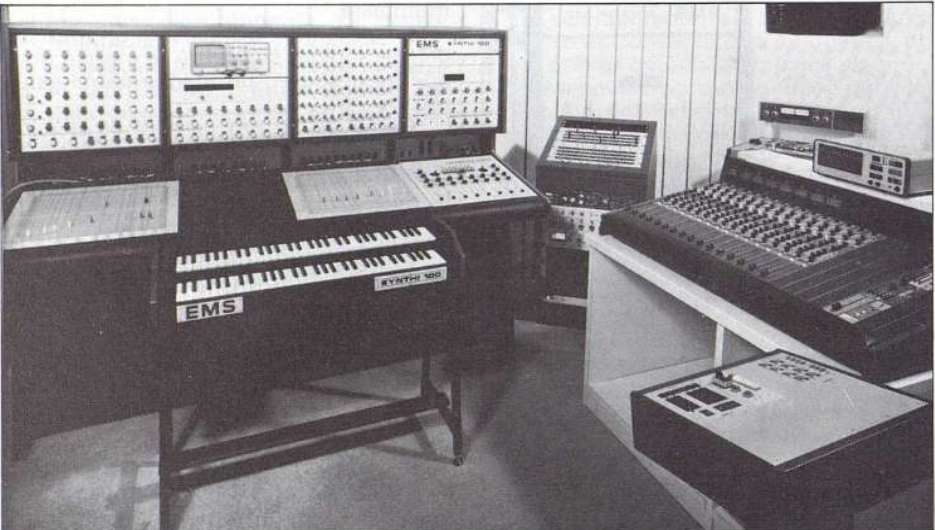
\includegraphics[width=0.7\textwidth]{GME_1984}
	\caption[Aspecto del GME de Cuenca en 1983.]{Aspecto del GME de Cuenca en 1983.}
	\label{fig:gme_1984}
\end{figure}

Fue inaugurado en 1983, dirigido por Pablo López de Osaba, director por aquel entonces del Conservatorio Profesional de Música, el Museo de Arte Abstracto Español y el festival de la Semana de Música Religiosa de Cuenca. El GME nació sin compositor asociado, siendo su primer técnico Leopoldo Amigo (1983--1990). En 1989 se contrata a Gabriel Brnčić como profesor de <<Teoría de la Composición>> y <<Teoría y Práctica de la Música con Medios Electroacústicos e Informáticos>>. Su labor se prolongará hasta 1998. Entre 1990 y 2006, el trabajo de Leopoldo Amigo será relevado por el del compositor Julio Sanz Vázquez. 

\begin{figure}
	\centering
	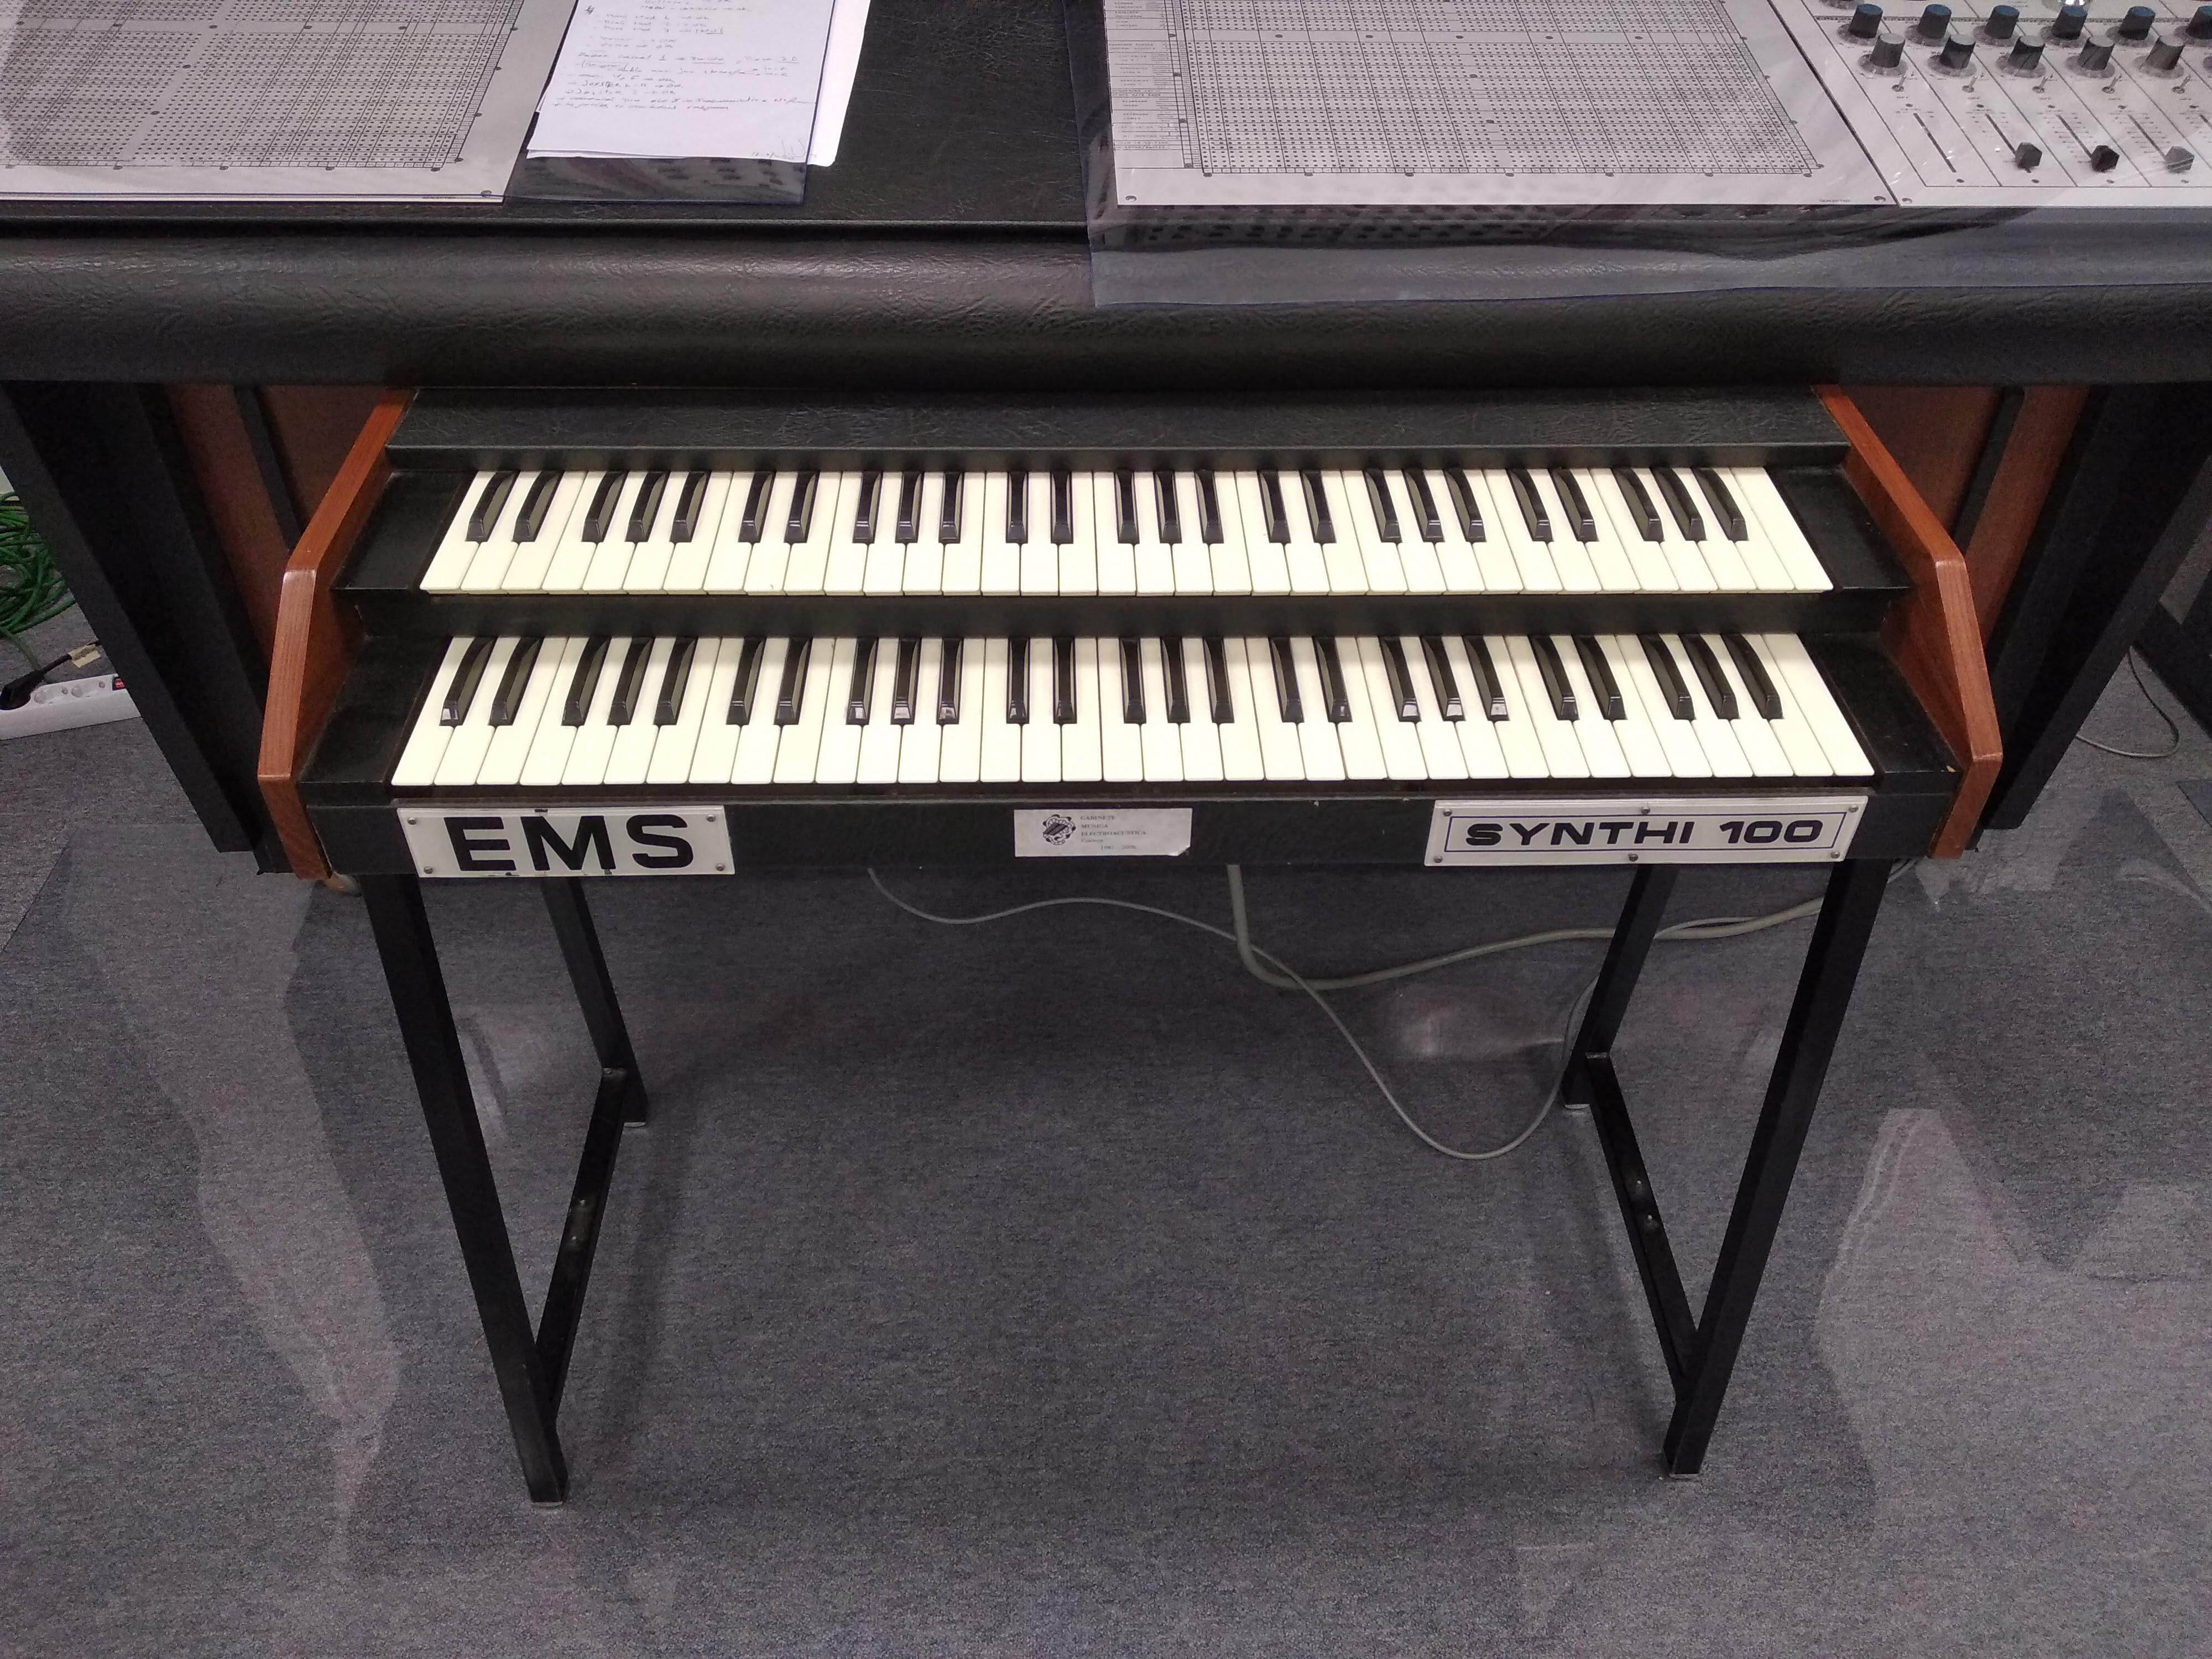
\includegraphics[width=0.7\textwidth]{teclado_EMS}
	\caption[Doble teclado EMS en Cuenca.]{Doble teclado EMS en Cuenca.}
	\label{fig:teclado_EMS}
\end{figure}

Los años en los que Gabriel ejerció su labor musical y magisterio coincidieron con los de mayor florecimiento de esta institución. Se organizaron los primeros cursos desde la oficialidad de un Conservatorio Profesional en España especializados en música electroacústica, así como conciertos mensuales en diversos espacios conquenses. Por sus instalaciones han pasado los más importantes compositores del momento, tanto por invitación como por iniciativa propia, para crear, dar conferencias o estrenar obras.

Tras la escisión del contrato de Gabriel Brnčić en 1998, el GME entró en un periodo de decadencia institucional (por motivos que no son objeto de este trabajo) que lo haría desaparecer a pesar de los esfuerzos llevados a cabo por su técnico Julio Sanz. Desde septiembre de 2006, momento en el que sus instalaciones fueron desmanteladas, un gran trabajo de recuperación y catalogación llega hasta nuestros días de la mano de la asociación AVADI (Audio Vídeo Arte Digital Interactivo), que nace con el objetivo de preservar el ingente material creado en el GME y luchar por la continuidad de la institución de cara al futuro. 

El elemento estrella del GME fue desde el principio el sintetizador EMS Synthi 100. Este modelo, heredero tecnológico del VCS3, alcanzó mucha popularidad en la década de los 70 y 80. Se caracteríza por la gran consola que lo alberga, compuesta de 4 paneles verticales y 3 horizontales. Va acompañado de un doble teclado (fig. \ref{fig:teclado_EMS}), si bien, según narra su técnico, Julio Sanz, apenas ha sido usado históricamente, ya que los compositores han usado el sintetizador principalmente para <<diseñar>> con él materiales sonoros que serían utilizados posteriormente en las mezclas y otros procesados.

\begin{figure}
	\centering
	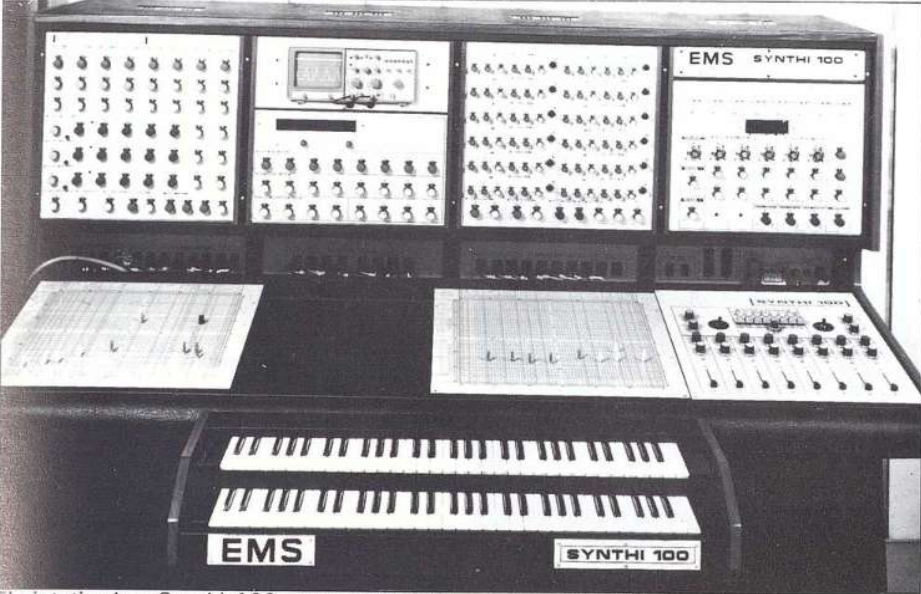
\includegraphics[width=0.7\textwidth]{synthi_1984}
	\caption[El Synthi 100 en el GME recién creado en 1983.]{El Synthi 100 en el GME recién creado en 1983.}
	\label{fig:synthi_1984}
\end{figure}

En él, todo es conectable con todo por medio de dos matrices de conexiones activadas por pines\footnote{Sobre esto me extenderé más a la hora de describir la emulación de estas matrices en \ref{sec:patchbay}.}. Llama la atención la gran cantidad de perillas que alberga, todas ellas numeradas con 10 niveles, quedando ocultos al usuario datos como el voltaje, frecuencia, amplitud, y otros parámetros a los que actualmente estamos acostumbrados a conocer de inmediato. La única forma de saber estos datos es analizándolos en el espectroscopio y el <<contador>> de frecuencia (fig. \ref{fig:frequency_counter}), pero estos módulos no dejan de ser <<analizadores>> de las señales que a ellos se les dirigen. No es posible conocer todos los datos de todos los módulos simultáneamente. Estas características han contribuido a crear un cierto halo de misterio alrededor del uso de este tipo de sintetizadores, pareciendo mágico el manejo de estos ante el espectador. Un inconveniente claro de este sistema es la dificultad en repetir un mismo resultado en dos momentos distintos. La naturaleza caótica de muchos de los procesos que implican la creación sonora hacen que pequeñas desviaciones de los valores deseados --incluso aquellas procedentes de agentes ajenos al Synthi y al usuario, como la temperatura o la humedad-- desemboquen en resultados sonoros completamente distintos.

\begin{figure}
	\centering
	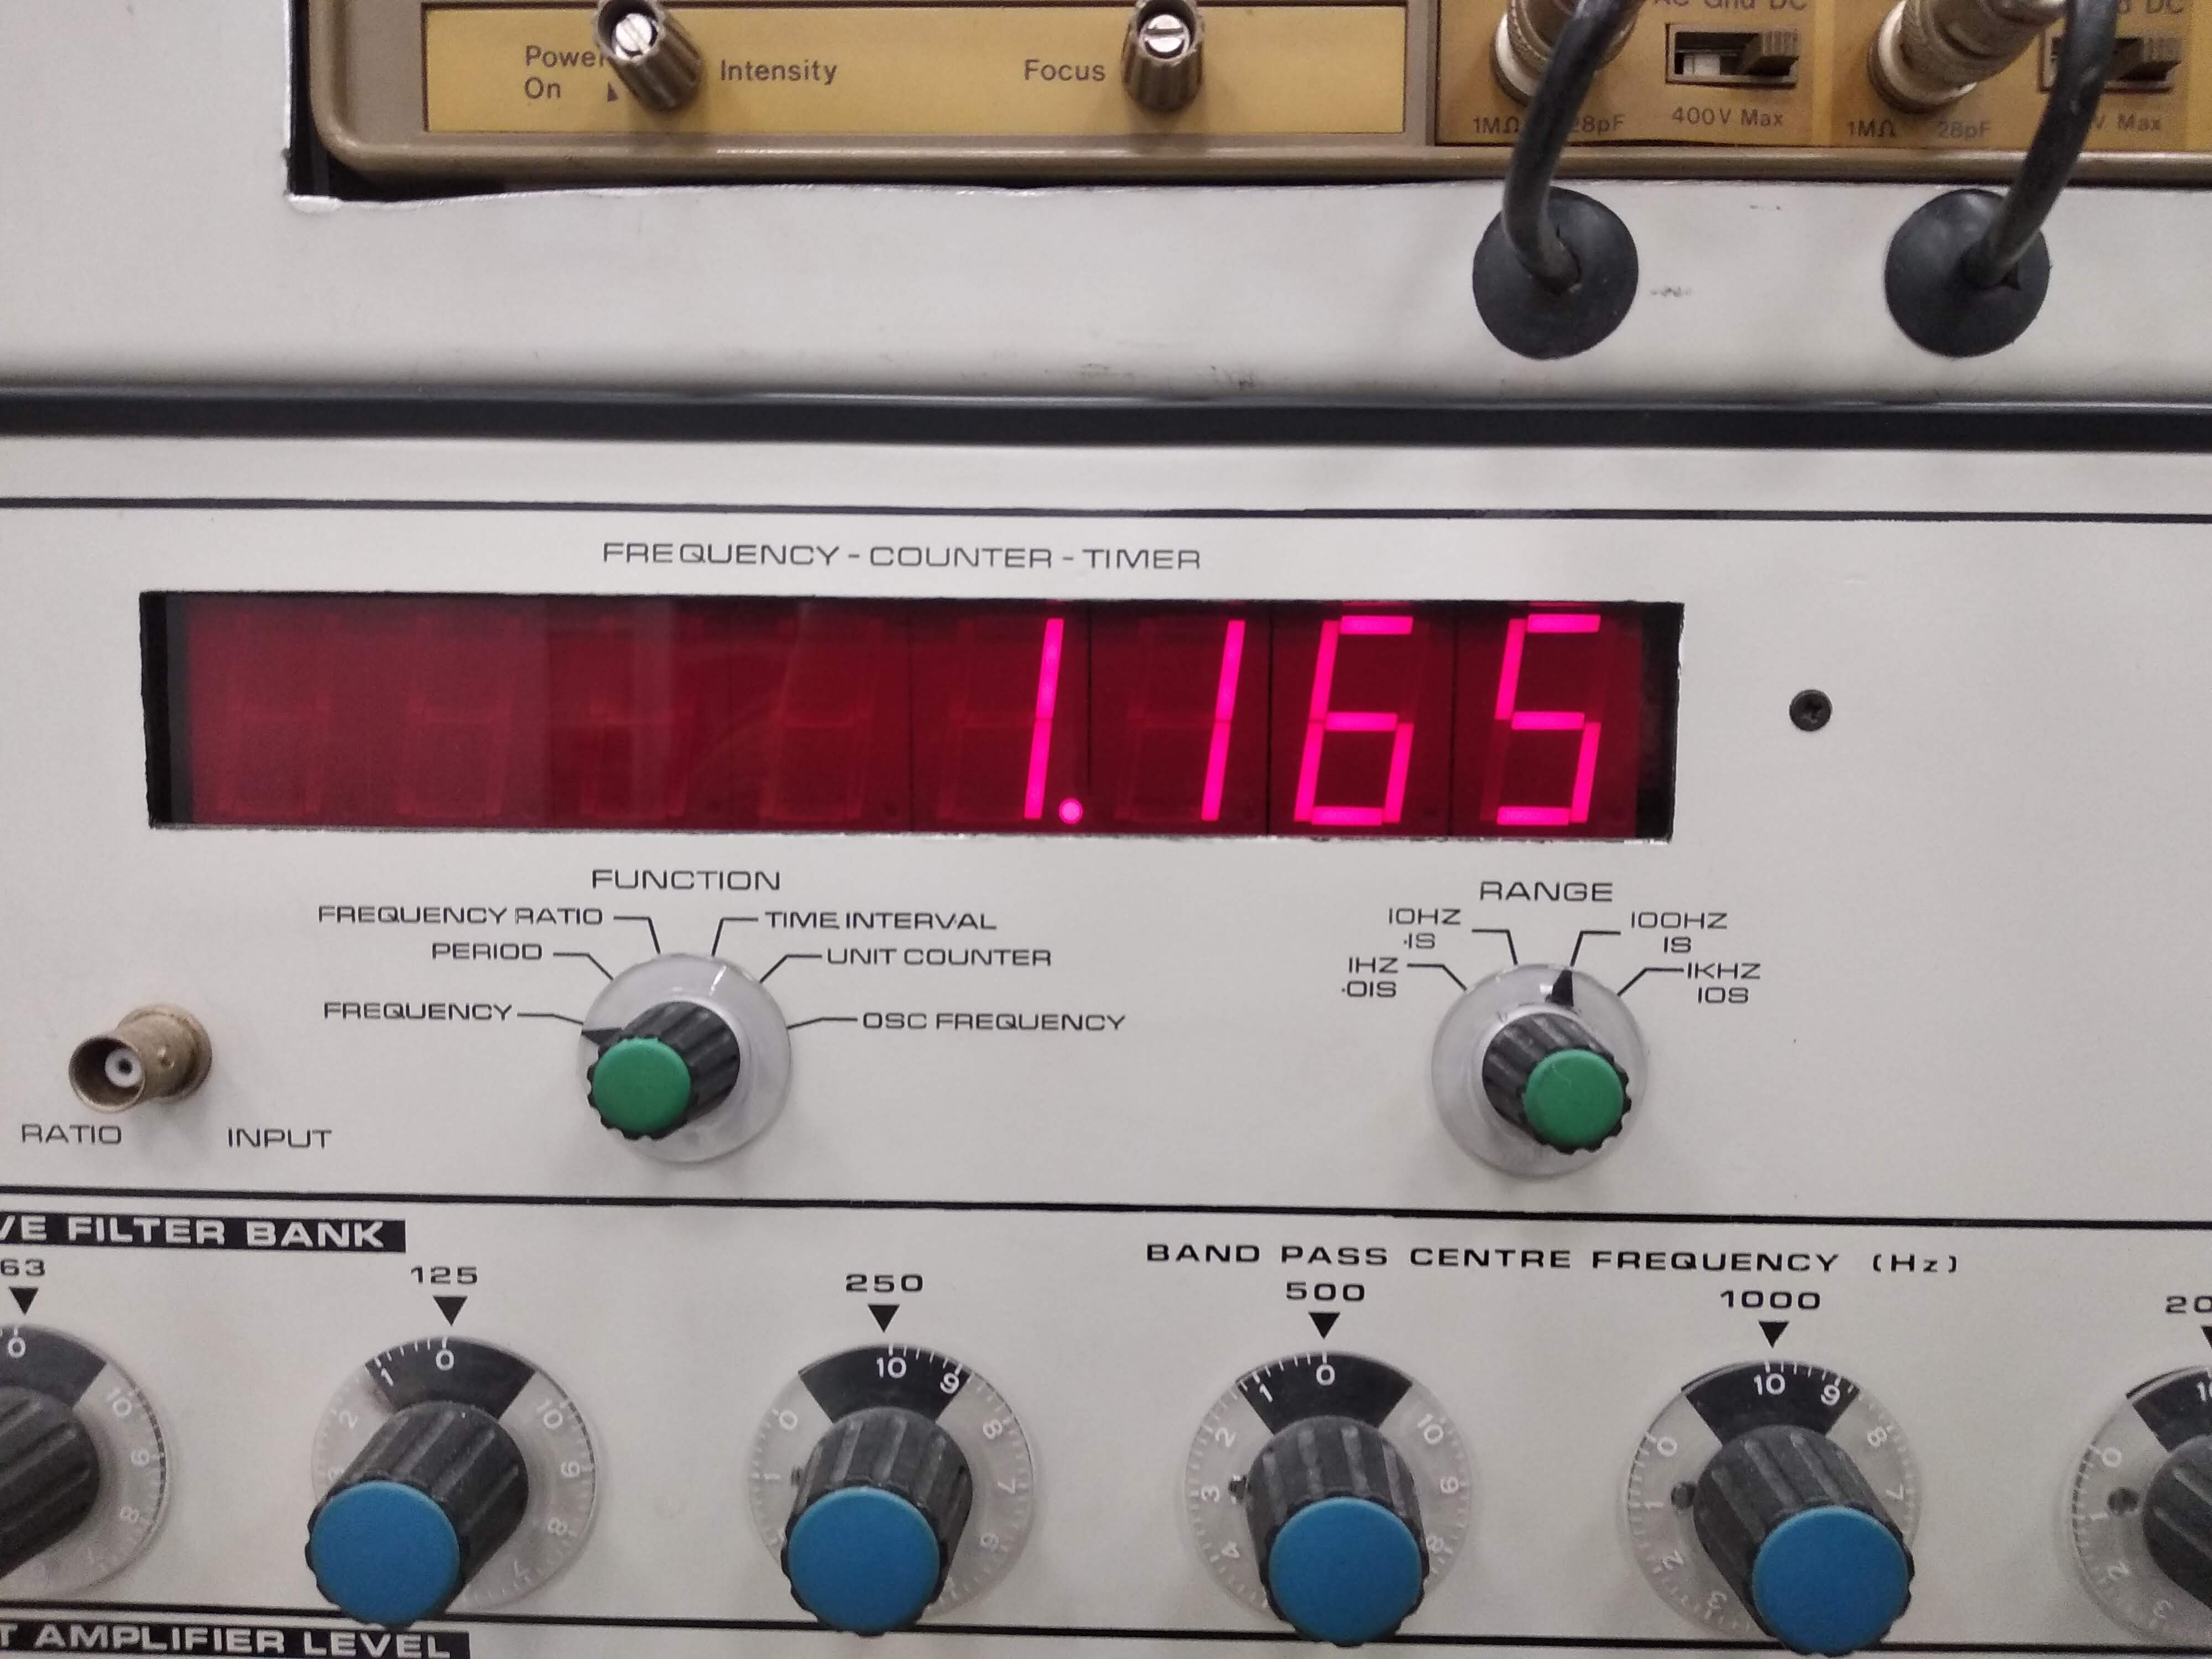
\includegraphics[width=0.7\textwidth]{frequency_counter}
	\caption[<<Contador>> de frecuencia.]{<<Contador>> de frecuencia.}
	\label{fig:frequency_counter}
\end{figure}


El sintetizador Synthi 100 está, en los momentos en los que se escribe esta memoria, en proceso de restauración. Con su recuperación se devuelve a la comunidad un instrumento histórico de un valor imponderable y que forma parte privilegiada de la historia del arte sonoro español. Actualmente, el GME está acogido por la Universidad de Castilla--La Mancha en Cuenca. Así, continua su andadura como la comenzó, en un centro público y disposición de todos.

\begin{figure}
	\centering
	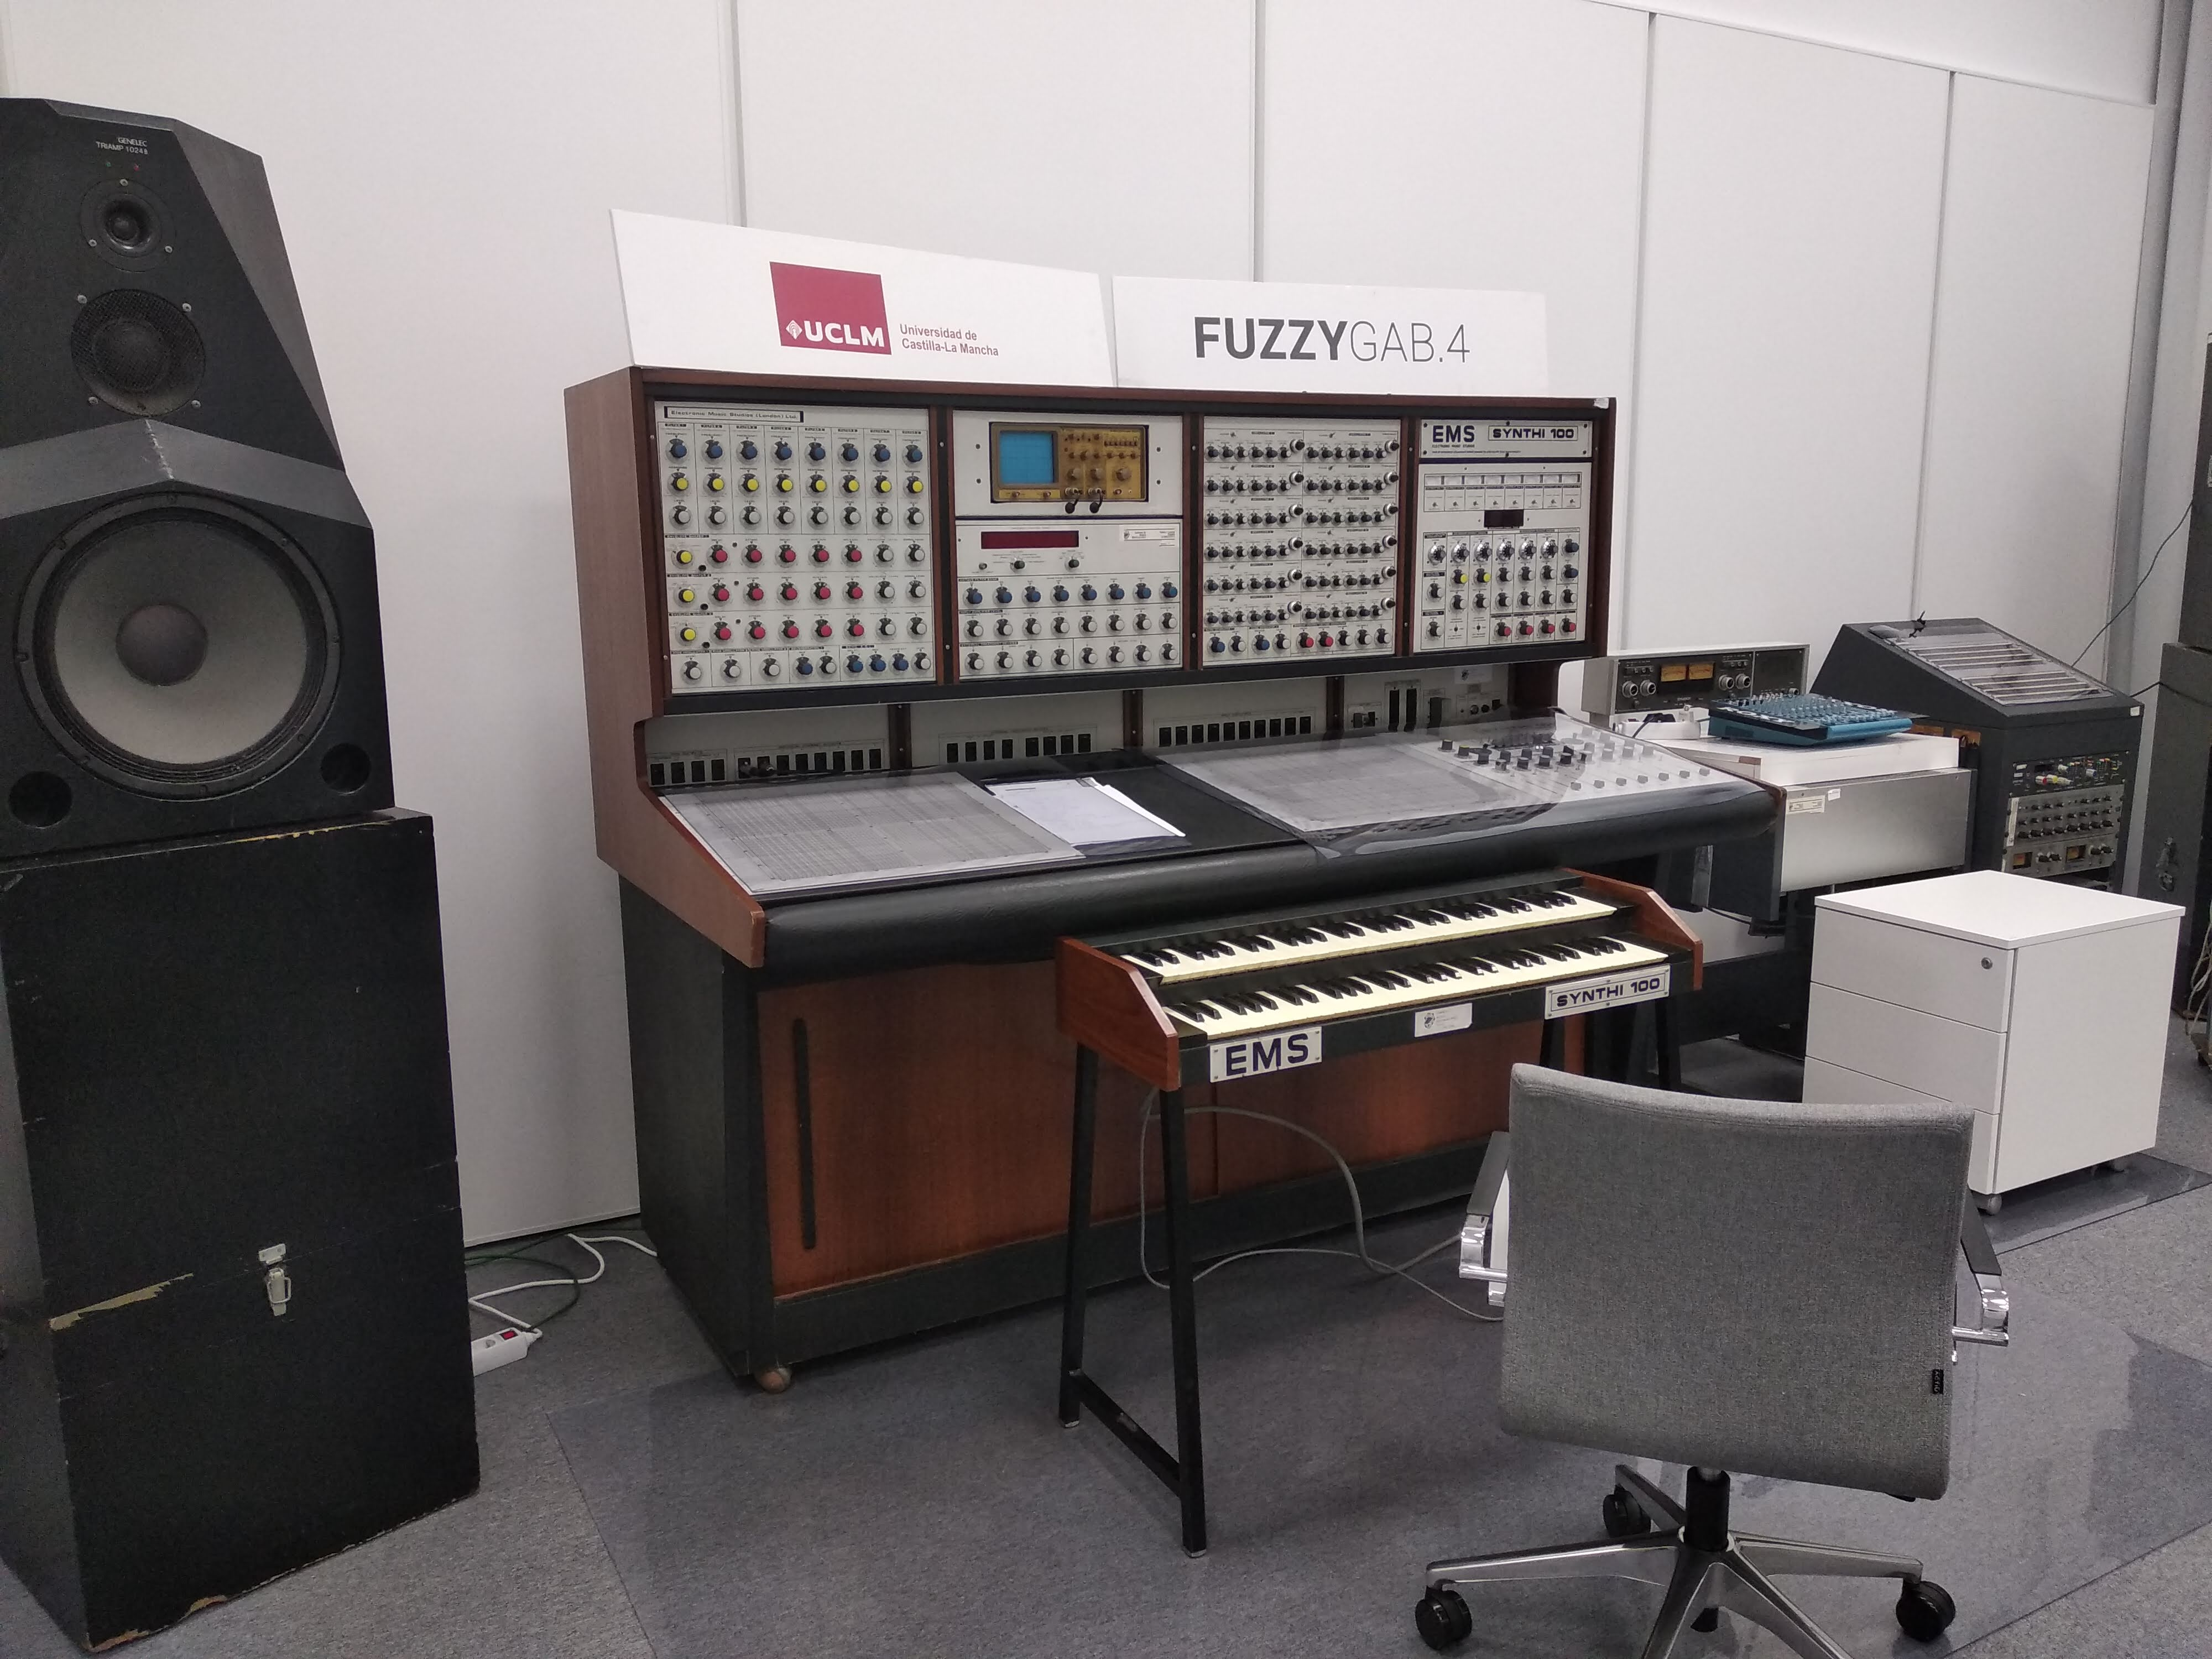
\includegraphics[width=0.7\textwidth]{synthi_GME_2020}
	\caption[El Synthi 100 en las instalaciones actuales del GME.]{El Synthi 100 en las instalaciones actuales del GME, en proceso de restauración.}
	\label{fig:synthi_GME_2020}
\end{figure}



